\section{MapReduce}

MapReduce est un patron d'architecture de développement informatique, inventé par Google, dans lequel sont effectués des calculs parallèles, et souvent distribués, de données potentiellement très volumineuses.
Ce module consiste en deux étapes :
\begin{itemize}
	\item map
	\item reduce
\end{itemize}

\subsubsection{Map}

Dans l'étape Map le nœud analyse un problème, le découpe en sous-problèmes, et les délègue à d'autres nœuds (qui peuvent en faire de même récursivement). Les sous-problèmes sont ensuite traités par les différents nœuds à l'aide de la fonction Reduce qui à un couple (clé, valeur) associe un ensemble de nouveaux couples (clé, valeur) :
\begin{equation}
map(key1,value1) → list(key2,value2)
\end{equation}


\subsubsection{Reduce}

l'étape Reduce, où les nœuds les plus bas font remonter leurs résultats au nœud parent qui les avait sollicités. Celui-ci calcule un résultat partiel à l'aide de la fonction Reduce (réduction) qui associe toutes les valeurs correspondantes à la même clé à une unique paire (clé, valeur). Puis il remonte l'information à son tour.
À la fin du processus, le nœud d'origine peut recomposer une réponse au problème qui lui avait été soumis :
\begin{equation}
reduce(key2,list(value2))→ list(value2)
\end{equation}



\begin{figure}[htpb]
	\centering
	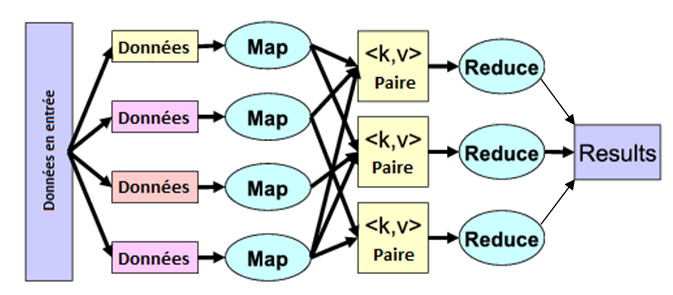
\includegraphics[scale = 0.5]{images/Mapreduce}
	\caption{Schéma de fonctionnement du MapReduce (source wikipedia)}
	\label{fig:MapReduce}
\end{figure}


Dans notre cas, l'étape Map ne découpe pas nos données en plusieurs groupes, cependant elle appelle plusieurs fois la fonction de calcul des prédictions sur plusieurs clés de paramètres différents tous indépendants les uns des autres. C'est pourquoi MapReduce est utilisé afin de lancer les calculs (qui sont importants et qui prennent du temps) en parallèle sur le cluster. 

%\subsubsection{Sensibilité et spécificité: explication}

%Au dessus, on a mentionné la sensibilité et la spécificité. mots d'une grande importance qui doivent être explicité afin de bien comprendre les résultats qui vous seront présenté aprés. 
%Ces termes vient d'une technique d'analyse statistique : \textit{Receiver Operating Characteristic curve}. Cette technique  permet de classé des résultats binaires (0 ou 1) en quatre groupes sous-jacent : 
%\begin{itemize}
%	\item vrai positif
%	\item faux positif
%	\item vrai négatif
%	\item faux négatif
%\end{itemize}

%Il s'agit donc de classer des résultats entre 0 ou 1 en comparant les scores obtenus avec les vrais. Ceci forme une courbe (voir figure X) qui représente la valeur de seuil selon la spécificité et la sensibilité. 
%Ces termes ont pour historique la détection sur des radars. Les radars sont dis sensibles si ils détectent correctement les événements importants parmi les événements qu'il a détecté. En revanche, un radar est spécifique si il ne détecte que des événements importants même si il n'en détecte pas beaucoup.  
%Dans notre cas, nous nous dirons sensibles si parmi tous les sujets classés malades, tous le sont, au contraire, nous serons spécifiques si nous avons classés peu de sujet malade mais ceux qui sont classés sont vraiment malade.
%La sensibilité correspond donc au taux de vrais positifs bien classés alors que la spécificité correspond au taux de vrais négatifs bien classés.  


%Maintenant que nous savons comment sont effectués les calculs et notre classification, passons maintenant a l'analyse de nos résultats. 
